\documentclass[english,]{article}
\usepackage{mathspec}
\setmainfont[]{TeX Gyre Pagella}
\PassOptionsToPackage{hyphens}{url} % url is loaded by hyperref
\usepackage[unicode=true]{hyperref}
\PassOptionsToPackage{usenames,dvipsnames}{color} % color is loaded by hyperref
\hypersetup{pdftitle={PhD thesis précis - Epidemiology of representations: an empirical approach},
            colorlinks=true,
            linkcolor=Maroon,
            citecolor=Blue,
            urlcolor=Blue,
            breaklinks=true}
\urlstyle{same}  % don't use monospace font for urls
\usepackage[a4paper]{geometry}
\usepackage{polyglossia}
\setmainlanguage[]{english}
\usepackage[style=authoryear-comp,
            uniquename=false,
            urldate=edtf,
            url=false,
            maxbibnames=20,
            giveninits=true,
            isbn=false]{biblatex}
\addbibresource{../content/bibliography-fixed.bib}
%\usepackage{csquotes}
%\DeclareLanguageMapping{french}{french-apa}
%\DefineBibliographyExtras{french}{\restorecommand\mkbibnamefamily}
\usepackage{graphicx}

\title{\large PhD thesis précis\\
\LARGE Epidemiology of representations :\\
an empirical approach}
\author{Sébastien Lerique\footnote{Previously: Centre d'Analyse et de Mathématique Sociales
  (CAMS, UMR 8557 EHESS-CNRS, Paris).
  Current: IXXI, Laboratoire de l'Informatique du Parallélisme (IXXI LIP, UMR 5668 Univ Lyon-ENS Lyon-Inria-CNRS-UCB Lyon 1).
  Email:
  \hbox{\href{mailto:sebastien.lerique@normalesup.org}{sebastien.lerique@normalesup.org}}.}\\
\hfill \\
Supervisor: Jean-Pierre Nadal\footnote{Centre d'Analyse et de
  Mathématique Sociales (CAMS, UMR 8557 EHESS-CNRS, Paris), and
  Laboratoire de Physique Statistique (LPS, UMR 8550 CNRS-ENS-UPMC-Univ.
  Paris Diderot, Paris). Email:
  \hbox{\href{mailto:jpnadal@ehess.fr}{jpnadal@ehess.fr}}}\\
Co-supervisor: Camille Roth\footnote{Centre d'Analyse et de
  Mathématique Sociales (CAMS, UMR 8557 EHESS-CNRS, Paris), and
  Centre Marc Bloch e.V. (UMIFRE 14 CNRS-MAEE, Berlin). Email:
  \hbox{\href{mailto:roth@cmb.hu-berlin.de}{roth@cmb.hu-berlin.de}}}}
\date{}

\begin{document}
\maketitle


\section{Introduction}
\label{sec:intro}

%Les années récentes voient se développer les tentatives de rapprochement entre sciences cognitives et sciences sociales.
%«Cognition sociale» et «Évolution culturelle» sont des exemples de thèmes émergents, abordés de manières multiples avec des apports de diverses disciplines.
%Cette thèse concerne un thème formalisé au milieu des années 90 par Dan Sperber.
%Dans une série d'articles novateurs rassemblés dans \textcite{sperber_explaining_1996}, ce dernier propose un programme de recherche aujourd'hui connu sous le nom de théorie de l'attraction culturelle (\emph{Cultural Attraction Theory} en anglais,
%noté CAT), visant à fournir un cadre commun dans lequel les sciences cognitives et les sciences sociales peuvent s'atteler à des questions interdisciplinaires.
%Ce programme part d'une ontologie ne comportant que des représentations mentales (celles des sciences cognitives), et des
%représentations publiques (l'expression hors du cerveau d'une représentation mentale).
%En proposant d'étudier la distribution et la dynamique d'évolution des représentations publiques circulant dans une société, Sperber développe un cadre permettant de combiner des travaux en anthropologie et en sciences cognitives pour l'étude des interactions entre évolution et culture.


Recent years have seen several attempts to bring cognitive science and social science together.
"Social cognition", "cognitive economy" and "cultural evolution" are examples of such fields having recently emerged, approached from multiple viewpoints and involving a variety of disciplines.
This thesis focuses on an approach formalised by Dan Sperber in the mid-nineties:
in a series of innovative articles gathered in \autocite{sperber_explaining_1996}, the author proposes a research program called \emph{Cultural Attraction Theory} (henceforth CAT), which aims to provide the cognitive and social sciences with a common framework to address interdisciplinary questions.
Since its initial introduction, this proposal has grown into one of the two main cognitively-inspired approaches to understanding the way a community's culture evolves over time due to mechanisms at the inter-individual level \autocites[the other approach being Standard Cultural Evolution,][]{cavalli-sforza_cultural_1981,boyd_culture_1985}.
These approaches, now "a booming cottage industry on the borders of evolutionary biology, archaeology, and biological anthropology" \autocite{sterelny_cultural_2017}, also propose a way of combining works from anthropology, cognitive science and evolutionary biology, disciplines that have remained isolated from one another for too long.

CAT is explicitly not a reduction of one of these fields to the other.
Nor does it claim to be a grand theory unifying all the disciplines studying life under one umbrella.
Instead, it creates bridges between cognitive science and anthropology so that the two can eventually work together in a common formulation of their questions.
To do so it proposes a general ontology where culture is thought of as a collection of representations:
representations can be either public, for instance a picture, a public speech, or this précis, or they can be mental (as those theorised by cognitive science), when someone interprets a public representation that they are perceiving.
%The ideas I am presenting in this précis, for instance, form mental representations in my mind.
%As I write them down, they appear to you as a public representation.
%If my writing is clear and accurate enough, the mental representations that you will form while reading this précis should be relatively close to the representations I have \autocite[p. 1]{sperber_explaining_1996}.
%In all likelihood, however, substantial change will have appeared in the process.
CAT suggests that the culture of a society can be modelled as a large dynamical system of representations being constantly interpreted into mental versions, and produced as new and transformed public representations.
A central question then appears:
given the significant changes that representations undergo each time they are interpreted and produced anew, how is it that culture can be so stable over time?
The cultural attraction approach answers this question by proposing that, due to the interaction of the cognitive processes and contextual factors at play when representations are transformed, the dynamical system that models a society should have attractors.
%In other words, it suggests that there are regions of representation space, more or less contingent on the state of culture at a point in time, towards which representations tend to come closer when they are transformed;
These \emph{cultural attractors} are CAT's main concept for explaining the stability of culture over time.



%The framework Sperber suggests starts from an ontology made only of "mental representations" (those from cognitive science) and their expressions in the outer world, "public representations".
%He then proposes to study the distribution of public representations that circulate in a society, and combine knowledge from cognitive science and anthropology to explain their evolution.
%As Sperber argues, this naturalistic approach builds on cognitive principles, is amenable to and can benefit from anthropological works, and allows interdisciplinary questions to be rephrased in terms of epidemiology of representations.
%For instance:
%what types of representations are only weakly transformed as they are interpreted and produced anew by successive people?
%Those representations, spreading wider than the others, become \emph{cultural}.
%Are they attractors for the interpretation-reproduction process of representations?
%If so, which cognitive modules are involved in the stability of such representations?


%La CAT a fait l'objet de développements théoriques récents avec une véritable modélisation mathématique \autocites[voir par exemple][]{claidiere_role_2007}{claidiere_how_2014}.
%Une communauté croissante aborde également les questions d'évolution et d'attraction culturelle avec des approches empiriques.
%Le paradigme des chaînes de transmissions artificielles, par exemple, a été beaucoup utilisé dans l'étude de l'évolution itérée du langage \autocite{tamariz_cultural_2016}.
%D'autres exemples de son utilisation sont l'étude de l'évolution de courtes boucles sonores modélisant une forme d'évolution musicale \autocite{maccallum_evolution_2012}, de la perception du risque dans des articles de presse \autocite{moussaid_amplification_2015}, ou de motifs visuels abstraits transmis par des babouins \autocite{claidiere_cultural_2014}.
%Une deuxième approche consiste à compiler un grand nombre de travaux anthropologiques ou historiques à propos d'un phénomène culturel bien précis, afin de reconstruire l'évolution d'un type de représentation et en analyser les tendances.
%C'est la méthode utilisée par \textcite{morin_how_2013} dans son étude de l'évolution, au cours des siècles, de la façon dont les portraits sont peints, et par \textcite{miton_universal_2015} dans leur étude de la pratique médicinale de la saignée.
%Une troisième approche consiste à récolter des données de communautés en ligne pour analyser la propagation de représentations dans des réseaux sociaux.
%Si bien les travaux pionniers de ce champ étaient basés sur des modèles d'exposition et de propagation atomique, où les objets d'étude étaient des entités simples et sans changements tels que des URLs \autocite[voir][ pour une discussion]{cointet_how_2007}, les travaux récents modélisent les représentations linguistiques avec une complexité croissante, et
%développent progressivement une description des phénomènes de transformations qu'un modèle de contenus atomiques ne peut pas
%atteindre.
%Plusieurs travaux étudiant de grandes bases de données de phrases réalistes ont déjà montré que la propagation ou la mémorisation de contenus linguistiques dépendra lourdement du contexte social \autocite{bakshy_social_2009}, du contenu sémantique et du style grammatical \autocite{danescu-niculescu-mizil_you_2012}, ainsi que de la situation de compétition avec d'autres contenus transmis \autocite{weng_competition_2012}.

%L'éventail des disciplines impliquées et la diversité des méthodes mises en place dans l'étude de ces questions sont un signe de la difficulté à récolter des données pertinentes pour l'étude de l'évolution culturelle.
%Les travaux cités ci-dessus développent plusieurs stratégies pour faire face à cet obstacle, mais laissent invariablement de côté certains aspects de la question:
%les chaînes de transmission utilisent généralement des représentations extrêmement simples;
%l'analyse quantitative de travaux anthropologiques ou historiques identifie des tendances pour lesquelles de nombreuses explications entrent en compétition;
%enfin, les modèles de propagation de contenus en ligne ont tendance à négliger le rôle de la cognition dans les phénomènes étudiés.

%Le fil directeur de cette thèse est le suivant:
%en capitalisant sur les possibilités actuelles des technologies informatiques, et en particulier les possibilités expérimentales des navigateurs web, il est possible de combiner les avantages de ces différentes techniques pour étendre le champ des questions d'évolution culturelle qui peuvent être étudiées empiriquement.
%Ce faisant, des sujets qui étaient jusque là restés au niveau théorique peuvent se manifester concrètement, ou même devenir des problèmes qu'il faudra résoudre pour avancer.
%Les travaux présentés dans cette thèse se concentrent sur un type particulier de représentation linguistique:
%de courts énoncés écrits, composés au plus de quelques phrases.
%Ce type de représentation est à la fois adapté à l'étude empirique (il est courant dans les réseaux sociaux en ligne, et relativement facile à utiliser dans des expériences contrôlées) et extrêmement versatile et varié. En prenant ces énoncés comme matériau principal, la présente thèse se propose de contribuer à l'étude empirique d'une des questions centrales de la CAT:
%l'existence d'attracteurs culturels, et leur pertinence dans l'étude de l'évolution culturelle à court terme.



The hypothesis of cultural attractors is interesting for at least two reasons.
On one side, it provides intelligibility into culture and its processes of change.
On the other side, it incorporates a central claim of the theory, namely that cognitive processes play an important role in the way culture evolves over time.
Empirically validating the existence of such attractors has thus become a major goal for the theory, but doing so has proved itself challenging.
%Indeed, it is not easy to collect quantitative data on the evolution of representations.
Up to now, empirical approaches to the question have fallen into three broad categories, each of which has some limitations.
The first is to simulate the evolution of representations in the laboratory, be it through iterated language evolution \autocite[see][for a review]{tamariz_cultural_2016}, or through so-called transmission chains used to study the evolution of objects such as short audio loops \autocite{maccallum_evolution_2012}, risk perception \autocite{moussaid_amplification_2015}, or abstract visual patterns transmitted by apes \autocite{claidiere_cultural_2014}.
%This approach allows for a detailed analysis of the transformations, but is often forced to use particularly simple (and thus non-ecological) representations in order to make the analysis tractable.
The second approach is to compile historical and anthropological works on a given subject to reconstitute the evolution of a type of representation as documented.
This technique has been used by \textcite{morin_how_2013} in his study of how painted portraits change over the centuries, and by \textcite{miton_universal_2015} in their examination of the practice of bloodletting.%, but has difficulties teasing apart the possible explanations for the evolutionary trajectories it observes.
The third approach is to study the evolution of representations in online social networks.
%up to now, however, works in this area have mostly overlooked the cognitive mechanisms at work in the processes of transformation.
%While earlier works were based on atomic propagation and exposure models where simple entities such as URLs and innovations were the central object \autocite[see][for a discussion]{cointet_how_2007}, this stream of research is increasingly modelling representations as deep objects with complexity of their own, improving on simpler virus-like models.
%Several works have now studied large quantities of meaningful sentences, showing that their propagation depends heavily on social context \autocite{bakshy_social_2009} and semantic content \autocite{danescu-niculescu-mizil_you_2012}, as well as on competition between items \autocite{weng_competition_2012}.

The wide array of disciplines studying these complementary questions, and the variety of techniques used in the process, testify to a major obstacle:
collecting relevant data in usable amounts to analyse cultural evolution is not easy.
Indeed, the works cited above invariably leave core aspects of the question aside:
transmission chains operate on extremely simple representations;
recompiling historical and anthropological works uncovers trends with many explanations competing for causality;
models of online content propagation overlook cognitive levels of explanation by and large.
It is possible, however, to combine the advantages of these techniques into new methods that significantly expand what empirical studies can tackle.
By applying the tools of psycholinguistics to the study of online communities on one side, and enabling transmission chains to benefit from widespread computing power and internet infrastructure on the other side, we are able to collect massive amounts of usable data for the empirical and quantitative study of out-of-laboratory epidemiology of representations.

Our practical goal in this thesis, then, is to introduce new empirical methods which combine the strengths of existing approaches, and can contribute to the validation of cultural attractors.
The more general goal is to contribute a detailed empirical study case to CAT, which we focus on linguistic utterances.
Indeed, linguistic traces of online interactions are readily available and easy to collect, such that it is possible to assemble data sets of useful size and quality for the study of this case.
Second, aside from providing an extremely versatile type of representation that makes the question of transformations interesting in itself, language is also at the core of several criticisms opposed to CAT.
Linguistic utterances are therefore a good use case to contribute to the debate surrounding CAT.
The thesis presents two novel exploratory methods for the evolution of linguistic utterances, in which the detailed transformations can be observed, and the relevance of attractors in explaining the changes can be assessed.
%Both methods are empirical and exploratory:
Both methods leave open the set of possible changes to observe, and work around the limitations of previously isolated approaches.
%The first method is an \emph{in vivo} approach, which combines data mining techniques with psycholinguistics in order to analyse the transformations of representations observed in online interactions.
%The approach thus relies on ecological data, but must face the high complexity of uncontrolled interactions between people in their everyday life.
%It must also find ways to deal with any missing data that was not collected as part of the digital traces.
%The second method is an \emph{in vitro} technique:
%it extends the current transmission chain approaches by creating a middle ground between the constraints of existing techniques, and manages to gather large sets of high-quality data with complex linguistic utterances, at an overall cost comparable to that of traditional laboratory transmission chains.
%Since it is a laboratory approach at the core, one can control the complexity of the utterances introduced and adapt them to the analysis planned.
%The downside is that participants in the experiment must be given a task to fulfil, which makes the experimental setting much less ecological than for \emph{in vivo} approaches.

Our experiments elicit significant and detailed biases in the way utterances are transformed, with overall trends that are consistent with the existence of attractors at the level of lexical word variables.
Aside from the raw results that we uncover about the transformation of utterances, we contend that these experiments are useful in two other ways.
First, they allow for a more precise formulation of the questions asked by CAT.
%The existence of cultural attractors in linguistic representations becomes a concrete question that can be evaluated using quantitative measures.
%Obstacles to the emergence of attraction, and the extent to which the cultural attraction picture describes the empirical evolution of utterances, can also be assessed.
Second, the experimental use of cultural attraction principles renders obvious the strengths and limitations of the approach for the case of linguistic utterances, and highlights new questions that should be explored by further research.
In particular, we shall see that the exact definition, and thus the existence, of a cultural attractor strongly depends on the dimension at which we describe linguistic utterances, %a question that cannot be decided at the principled level.
%We will also see that the meaning of utterances is a crucial factor in the evolution of short utterances,
and that an account of how meaning is understood in context must be included in the theory to make further progress in the linguistic case.


\section{Word substitutions in blogspace quotations}
\label{sec:bcp}

Our first case study introduces a data analysis approach which takes advantage of the ever-increasing avalanche of available digital footprints since the 2000's.
Indeed, tools and computing power to analyse such data are now widespread, and the body of research aimed at describing online communities and content is growing accordingly.
For instance, the propagation of cultural artefacts across social networks has been studied in blogspace \autocite{gruhl_information_2004} and in emails \autocite{liben-nowell_tracing_2008};
\textcite{cointet_socio-semantic_2009} described the reciprocal influence between the social network topology and the distribution of issues;
\textcite{leskovec_meme-tracking_2009} detailed the characteristic times and diffusion cycles both within these social networks and with respect to the topical dynamics of news media, and \textcite{danescu-niculescu-mizil_you_2012} studied the characteristics of particularly memorable quotes that circulate in those networks.
By mining similar data sets in a cognitive-aware manner, we believe it is possible to connect the field of cultural evolution with psycholinguistics, and thus advance the testing of cultural attractors.

To do so we analyse how quotes in blogs and media outlets are modified when they are copied from website to website.
Indeed, such public representations should normally not change as they spread on the Web (as opposed to more elaborate expressions or opinions, not identified as quoted utterances), but empirical observation shows that they are in fact occasionally transformed \autocite{simmons_memes_2011}:
authors spontaneously transform quotes, not only cropping them but also replacing words.
For instance the quote "we will not be scared of these cowards" (a substring of a quote from former Pakistani President Asif Ali Zardari) is also found as "we will not be \textbf{afraid} of these cowards".
More meaningful changes often happen too, such as the transformation of McCain's "I admire Senator Obama and his accomplishments" during the 2008 US presidential campaign, into "I \textbf{respect} Senator Obama and his accomplishments".
Since authors are implicitly required to copy quotes exactly, we can assume that most transformations, especially simple ones such as those shown above, are the result of automatic (i.e. hard to control) low-level cognitive biases of the authors.
%Ces représentations publiques ne devraient normalement pas être modifiées lors de leur propagation en ligne (contrainte absente pour des segments de texte non explicitement identifiées comme du discours direct, par exemple une opinion ou un argumentaire résumés), mais l'observation empirique indique qu'elles sont effectivement transformées régulièrement \autocite{simmons_memes_2011}:
%les auteurs d'articles en ligne transforment certaines citations spontanément, sans se limiter à un simple rognage de l'original, mais également en remplaçant certains mots.
%Par exemple, on trouve la citation «We will not be scared of these cowards»\footnote{«Nous ne serons pas effrayés par ces lâches».
%Ici et dans la suite, les traductions sont miennes.}
%(extraite d'une citation de l'ancien président pakistanais Asif Ali Zardari) sous plusieurs formes, l'une d'entre elles étant «We will not be \emph{afraid} of these cowards»\footnote{«Nous n'aurons pas peur de ces lâches».}.
%Des transformations plus significatives apparaissent également, par exemple la phrase «I admire Senator Obama and his accomplishments»\footnote{«J'admire le sénateur Obama et ses accomplissements»}, prononcée par McCain au moment de la campagne de 2008 pour les présidentielles aux États-Unis, apparaît aussi sous la forme «I \emph{respect} Senator Obama and his accomplishments»\footnote{«Je respecte le sénateur Obama et ses accomplissements»}.
%Puisque les auteurs de ces articles ont l'obligation implicite de rapporter de telles citations de façon exacte, on peut supposer que la plupart de ces transformations (et en particulier les plus simples, comme celles montrées ici) sont l'effet de biais cognitifs automatiques et difficiles à contrôler.

We thus ask the following question: given such representations that seem to evolve precisely because of the kind of automatic cognitive biases evoked in Cultural Attraction Theory, do cultural attractors appear, and if so how do cognitive biases participate in them?
We chose to restrict our analysis to substitutions (i.e., one word being replaced by another), both to keep the analysis tractable and because of missing information in our data set.\footnote{
As explained in the thesis, source-destination links between quotes must be inferred from the data set, an operation which is much more reliable if we restrict our analysis to substitutions.
%This also impedes us from observing the effect of accumulated transformations in the long term, limiting our results to a view of the individual evolutionary step.
}
While this limits the scope of our results to the particular data set we use, the methodological point we also make is left intact.
%On peut alors poser la question suivante:
%étant donné que ces représentations publiques semblent évoluer au moins pour partie à cause de biais cognitifs, c'est-à-dire par un mécanisme que la CAT considère comme fondamental pour l'évolution culturelle et l'émergence d'attracteurs culturels, peut-on observer de tels attracteurs dans la dynamique d'évolution des citations, et si oui comment les biais cognitifs y participent?
%Ce chapitre se concentre sur les substitutions de mot à mot, à la fois pour rendre l'analyse possible techniquement et pour remédier au manque de certaines informations dans le jeu de données utilisé.
%Si cette restriction limite quelque peu la portée des résultats obtenus, l'argument méthodologique que ce chapitre nous permettra de faire reste intact.
By characterizing words using 6 well-studied features, we show that authors preferentially substitute words known for being harder to recall:
most prominently words with low frequency \autocite{gregg_word_1976}, learned later \autocite{dewhurst_separate_1998}, or made up of more letters \autocite{nickels_dissociating_2004}, both globally and in comparison to the sentence they appear in.
%This result is obtained by comparing the observed behaviour to what would happen if targets were picked randomly in the sentences.
Further characterizing the substitutions by examining the variation of word features from disappearing to appearing words, we show:
(a) that the operation is contractile on average, that is, a transformation will usually bring words closer to an attractor point on each feature, much more than what a semantically plausible but random process would do;
(b) that authors produce words that are easier to remember than the synonyms of the disappearing word (a fact that is reflected in the position of the attraction point).
%En codant les mots des citations avec six variables lexicales dont les effets sont bien connus en psycholinguistique, nous identifions ce qui rend une substitution plus probable dans une citation, et caractérisons la façon dont les mots sont transformés lors d'une substitution à l'aide de deux mesures principales:
%la susceptibilité à être substitué, et la variation lors d'une substitution.
In other words, the substitutions behave consistently with the existence of feature-specific attractors, and their behaviour cannot be explained by assuming that words are simply replaced by random synonyms.

Unfortunately we do not actually observe quotes converging on a global scale towards attractors in their various dimensions, as the limits of the data set do not allow us to infer chains of substitutions.
Furthermore, substitutions themselves are not the only type of transformation at work in the data set (however both these points are addressed in the next chapter).
Nonetheless, these findings (a) bring light to this simple type of transformation, and (b) elicit biases which are consistent with known psycholinguistic effects, with the hypothesis of cultural attractors in representations from everyday life, and with the hypothesis of lineage specificity which the iterated learning literature discusses \autocites{claidiere_cultural_2014,cornish_systems_2013}.
%Bien que les transformations étudiées dans ce chapitre ne sont pas les seules à jouer dans l'évolution des citations, ces résultats sont en accord, d'un côté, avec l'hypothèse de l'existence d'attracteurs spécifiques à chaque variable linguistique dans le processus d'évolution des citations, et de l'autre, avec les effets connus de ces variables lexicales en psycholinguistique.
As a whole, this first study can be viewed as analysing part of the transmission step operating in transmission chains of artificial languages like those studied by \textcite{kirby_cumulative_2008}, yet with natural language out of the laboratory.
It works by successfully applying knowledge from cognitive science to real-life complex data, a task that remains a challenge in the study of cultural evolution.
More broadly, we believe that applying such data mining tools to manage the complexity of real-life data is a promising approach for the joint analysis of cognitive science and culture.
%Cette approche, qui combine psycholinguistique et exploration d'une grande base de données, permet de mettre en lumière un certain nombre de biais concordants avec les effets connus des variables lexicales utilisées.

%En particulier, les mots connus pour être plus difficiles à rappeler dans des expériences de rappel de listes de mots en laboratoire (c'est-à-dire les mots moins fréquents, appris à un âge plus tardif, ou sémantiquement moins faciles à identifier) ont tendance à être plus substitués;
%deuxièmement, les mots plus faciles à produire dans ces tâches (c'est-à-dire les mots plus fréquents, appris plus jeune, ou faciles à identifier sémantiquement) sont aussi plus souvent introduits en remplacement.
%Le motif particulier des substitutions observées montre également que ces transformations introduisent des mots qui sont en moyenne plus proches d'une valeur spécifique à chaque variable lexicale, valeur qui agit comme un attracteur sur cette dimension.
%Ces résultats sont valables également lorsqu'on prend en compte le contexte fourni par une citation:
%un mot plus difficile à rappeler par rapport aux autres mots de la citation dans laquelle il apparaît sera plus souvent substitué;
%de même, un mot plus facile à rappeler par rapport au reste de la phrase sera plus souvent inséré en remplacement.


%Autrement dit, l'analyse présentée dans ce chapitre soutient l'hypothèse selon laquelle des attracteurs culturels peuvent résulter de l'interaction de biais cognitifs individuels dans l'interprétation et la reproduction de représentations \autocite{lerique_semantic_2017}.
%Au niveau méthodologique, la démarche suivie ici, validée par de nombreuses vérifications manuelles, montre aussi qu'il est possible d'extraire rigoureusement des motifs de transformation des énoncés dans des données venues de la vie réelle, et de relier ces motifs à des effets connus de la psycholinguistique en laboratoire.
%L'analyse de telles données plus écologiques nécessite de faire face à la complexité inhérente des interactions humaines dans un cadre non contraint, mais un choix judicieux de simplifications permet de rendre la démarche possible en pratique.


\section{Transformations in large-scale transmission chains}
\label{sec:gistr}

Our second case study aims to remedy several caveats of the previous chapter by studying the evolution of short utterances in a controlled experimental setting.
Indeed, the online corpus only let us examine simple transformations, remained at the low level of lexical properties such as word frequency and age of acquisition, and did not let us identify chains of transformations.
In this chapter therefore, we develop a novel online and controlled experimental setting: while the situation will be somewhat less ecological, it will allow for the collection of all the necessary data for a deeper analysis.

Here too, our approach is exploratory:
our goal is to construct a descriptive model of the process that can bring insight into why utterances change the way they do, and how such observations can be connected to current knowledge in linguistics, on one side, and to the broader cultural evolution frameworks, on the other.
Indeed, current knowledge of the transformation of utterances is quite partial:
laboratory transmission chains show that a number of high-level biases appear in the transmission of purposefully constructed complex stories, but do not explain in detail how such trends come about.
On the other hand, the psycholinguistics literature on sentence recall shows that there are important semantic and syntactic effects in the way sentences are reformulated, but they do so on extremely simple types of content that make it difficult to generalise results.
There seems to be a missing link that could connect the high-level effects that are observed in transmission chains of complex stories with the lower-level processes that are known to act in the recall of simple sentences.
A descriptive model of transformations would go a long way in creating this link, and would make it much easier to explain the overall evolution of utterances in terms of lower-level cognitive mechanisms.

In order to collect a sufficient amount of quality data, we chose to run a set of transmission chain experiments on an online platform developed for the purpose:
indeed, after an initial development phase, the web-based experiment approach lets us collect large amounts of data in short periods of time, while maintaining a level of control similar to that of laboratory experiments \autocite{lerique_gistr_2016}. 
In particular, it frees us from the limits of previous empirical approaches by combining three important properties:
\begin{itemize}
  \item the use of realistic and ecological pieces of linguistic content (as opposed to the simplified sentences used in psycholinguistics, and to the minimal content types used in transmission chains);
  \item complete control over the data-generation process and its collection (as opposed to the analysis of large databases coming from online sources such as social media);
  \item the possibility for computational analysis, thanks to large-scale collection of quality data (contrary to most setups using realistic content), and the development of a specific technique for analysing transmission chains.
\end{itemize}

This approach let us run several large scale transmission chain experiments (up to 10 reformulations of each initial sentence with 140 participants), collecting complex and very high quality transformations (around 1\% percent total spam rate) of a varied set of initial utterances.
%The experiment is available to subjects as a website, on which participants register, answer a preliminary questionnaire, then train for and complete the main task:
%L'expérience se présente sous la forme d'un site web sur lequel les sujets s'inscrivent, répondent à un questionnaire initial, s'entraînent puis complètent la tâche principale:
%subjects are asked to repeatedly memorise and rewrite short utterances as accurately as possible.
%il s'agit de lire un énoncé écrit, de s'en souvenir pendant une phase d'attente, puis de le réécrire aussi précisément que possible.
%Each subject thus reformulates between 25 and 50 utterances, making experiments last between 40 minutes and an hour.
%Chaque sujet reformule ainsi entre 25 et 50 énoncés, pour une expérience durant entre 40 minutes et une heure.
%A specific challenge of the web experiment procedure is the design of the interface.
%Un défi spécifique au procédé d'expérimentation en ligne est le design de l'interface:
%There is no opportunity for a face-to-face walk-through of the experiment or for
%questions, and subtle changes in the way the interface reacts to actions can lead subjects to interpret
%a signal where none was intended, or conversely to not notice an important message. The time of the
%subjects is not booked, and not having to travel to the laboratory or to talk to someone renders the
%interaction free of any commitment and generally more consumable: subjects can leave whenever
%they want, without having to feel bad about it (the only cost being the loss of their reward). The lack
%of human interaction with the experimenter also removes a natural incentive for subjects to take
%their time and perform according to what the experimenter in front of them explained. Combined
%together, these factors mean that if the interface is strenuous or ambiguous in any way, subjects
%will often pick the interpretations that make the process faster and either complete the experiment
%with minimal engagement or drop out. Redacting detailed textual instructions often makes matters
%worse. Instead, the interface must lead the subjects through the necessary explanations while re-
%maining enjoyable, and must be unambiguous while still hinting towards the expected behaviour at
%the right moment, either through subtle interface reactions or through explicit contextual aids.
%en effet, n'ayant pas d'interlocuteur physique dont la présence pourrait encourager à prêter attention où à poser des questions, les sujets peuvent facilement interpréter certains aspects de l'interface d'une façon inattendue.
%Il est donc particulièrement important de créer une interface sans ambigüités qui accompagne les sujets dans leur concentration et leur compréhension de la tâche, et ce afin qu'ils restent consciencieux et produisent des phrases de la meilleure qualité possible.
%A sustained effort in this area let us reach very high quality data (around 1\% percent total spam rate), letting us gather transmission chains of up to 10 reformulations, based on a sufficiently varied and complex set of start utterances to trigger substantial transformations.
%Un effort soutenu en ce sens nous a permis d'atteindre un taux de qualité excellent (aux environs de 1\% de spam au total).
%On obtient alors des chaînes de transmission pouvant aller jusqu'à 10 reformulations, basées sur un jeu de phrases varié et suffisamment complexe pour se prêter à des transformations substantielles.
Our analysis is then geared towards creating an intermediary representation of the effect of transformations on utterances, one that is at a midpoint between the low-level of word features and the high-level of category contrasts, and which can be usefully modelled to better understand the evolution of utterance chains.

To this end we rely on a sequence alignment algorithm originating in bioinformatics, which we extend to the linguistic case,
%initially developed in order to align sequences of DNA for the detection of relationships between species, this algorithm infers the most probable transformation that relates two sequences of items which can be compared pairwise.
%We begin by adapting the algorithm to the linguistic case by considering sequences of words, then extend it to make it capable of accounting for synonyms and detecting exchanges between separate parts of an utterance.
and further develop to be aware of synonyms and exchanges between separate parts of an utterance.
Once correctly parametrised using a supervised training technique, we can decompose the transformations that subjects introduce into a series of elementary operations on each word or block of words:
insertion, deletion, replacement, or exchange between subparts.
This decomposition allows us to create a descriptive model and visualisations which are both general and precise in what they capture of the evolution of utterances along chains. Figure \ref{fig:lineage} illustrates such a visualisation.

\begin{figure}[!ht]
	\centering
	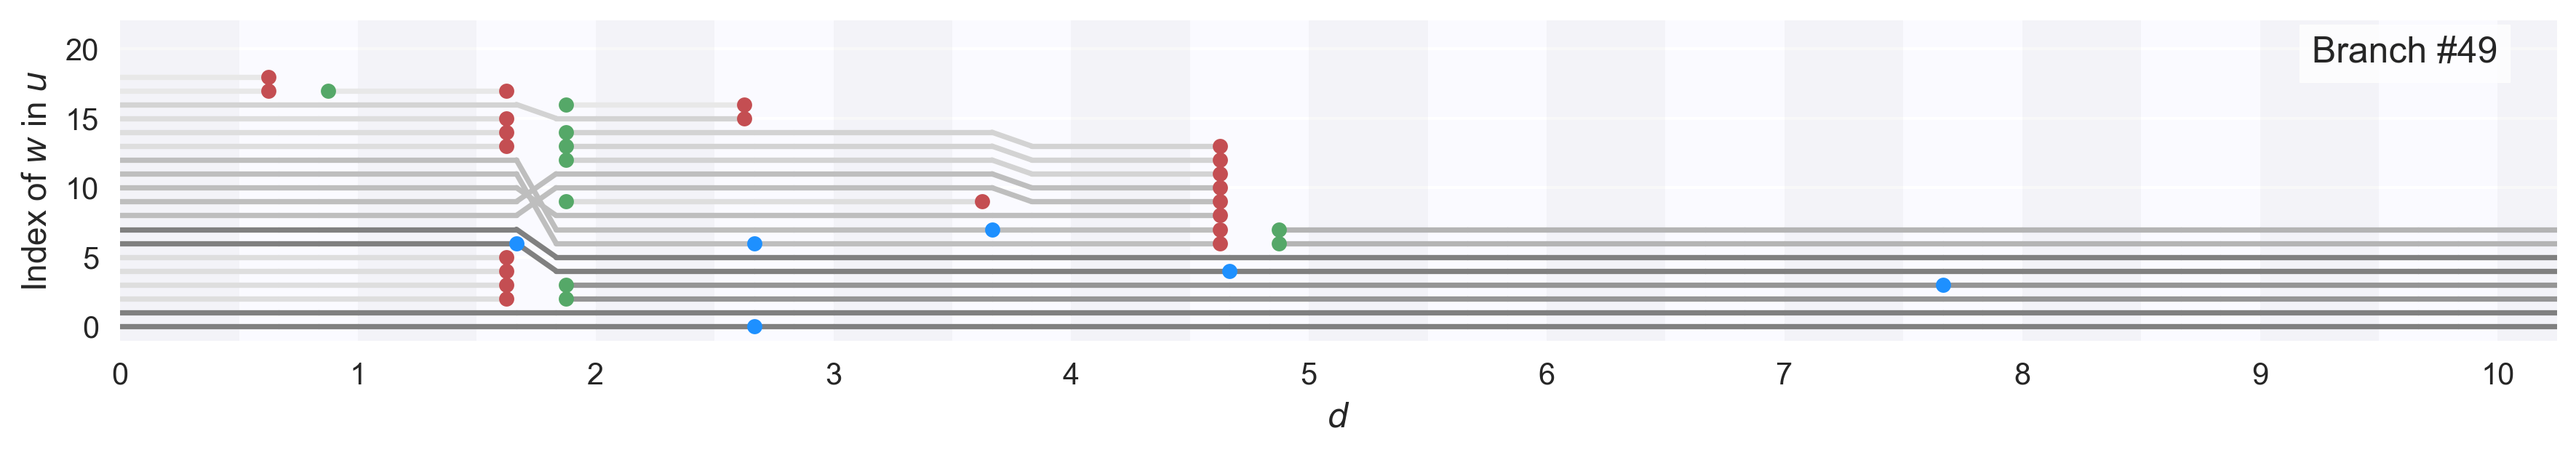
\includegraphics[width=\linewidth]{lineage-tree-4.png}
	\caption{\emph{Evolution diagram of an utterance along a chain.}
	The horizontal axis is the depth in the branch, and the vertical axis is the index of each word in its utterance.
	A grey line represents a word lineage along the branch, and the darkness of the line corresponds to lifetime of that word (darker lines indicate words that survive longer across transformations).
	At each depth, the darker background band indicates what the subject sees, and the lighter band indicates the transformation that the subject made.
	Inside lighter bands: red dots are word deletions, green dots are word insertions, blue dots are word replacements, and exchanges can be seen when bundles of lines cross each other.
	The initial utterance is «At Dover, the finale of the bailiffs' convention. Their duties, said a speaker, are "delicate, dangerous, and insufficiently compensated."»\autocite{feneon_novels_2007};
	the final utterance is «in Dover at the bailiffs conventions something happened».}
	\label{fig:lineage}
\end{figure}

We then quantitatively characterize the individual behaviour of each operation, as well as the dependencies between operations.
Indeed, operations strongly depend on each other (e.g., insertions appear to make up in size for some of the deletions, while still introducing substantial change; in turn, deletions behave as a gating mechanism for other operations), and their prevalence also depends on the length of, and their position in, each utterance (longer utterances receive more operations; replacements preferentially target the interior of utterances, and insertions and deletions target the second half of utterances).
%Nous caractérisons alors le comportement individuel de chaque opération ainsi que les interdépendances entre opérations, montrant que les suppressions et insertions de mots touchent des blocs entiers plutôt que des mots individuels, et que toutes les opérations dépendent fortement de la longueur de l'énoncé initial ainsi que de la position à laquelle elles opèrent (par exemple, les insertions et les suppressions sont plus probables dans la deuxième moitié d'un énoncé, et beaucoup plus fréquentes pour des énoncés plus longs).
%Les remplacements sont relativement indépendants des autres opérations.
%On observe en revanche que les suppressions agissent comme un déclencheur pour plus de transformations, et que les insertions tentent souvent de réparer les dégâts créés par une délétion en bloc en introduisant un nombre comparable de nouveaux mots à la même position dans l'énoncé.
The behaviour of each of these operations is also consistent with the biases identified in the previous chapter in terms of word features.%, and the new results complement the previous ones to offer a much more complete view of the process at work.
%the susceptibilities for being targeted by deletion or replacement, and appearing by insertion or replacement, closely complemented each other, in accordance with the hypothesis of an attractor at the lexical level.
Finally, we observe the overall evolution of the lexical makeup of utterances, which illustrates the attraction pattern on each lexical feature as previously hypothesized (see figure \ref{fig:branchevo}).
%Enfin, nous transposons la démarche effectuée au chapitre précédent aux données de cette expérience, et confirmons les résultats:
%les mots peu fréquents, appris à un âge plus tardif, plus longs ou sémantiquement plus difficiles à identifier sont en moyenne plus souvent supprimés ou remplacés, en faveur de mots plus faciles à rappeler.
%Contrairement aux données issues de blogs nous avons ici accès aux chaînes de transmission, nous permettant d'observer l'effet accumulé de ces transformations sur les variables lexicales.
%Les résultats attendus et observés sont illustrés dans la figure \ref{fig:branchevo}:
%les énoncés sont progressivement transformés le long des chaînes vers des versions utilisant des mots connus pour être plus faciles à rappeler dans des tâches de rappel en laboratoire, indiquant que des biais cognitifs de bas niveau pourraient en être responsables.

\begin{figure}[!ht]
	\centering
	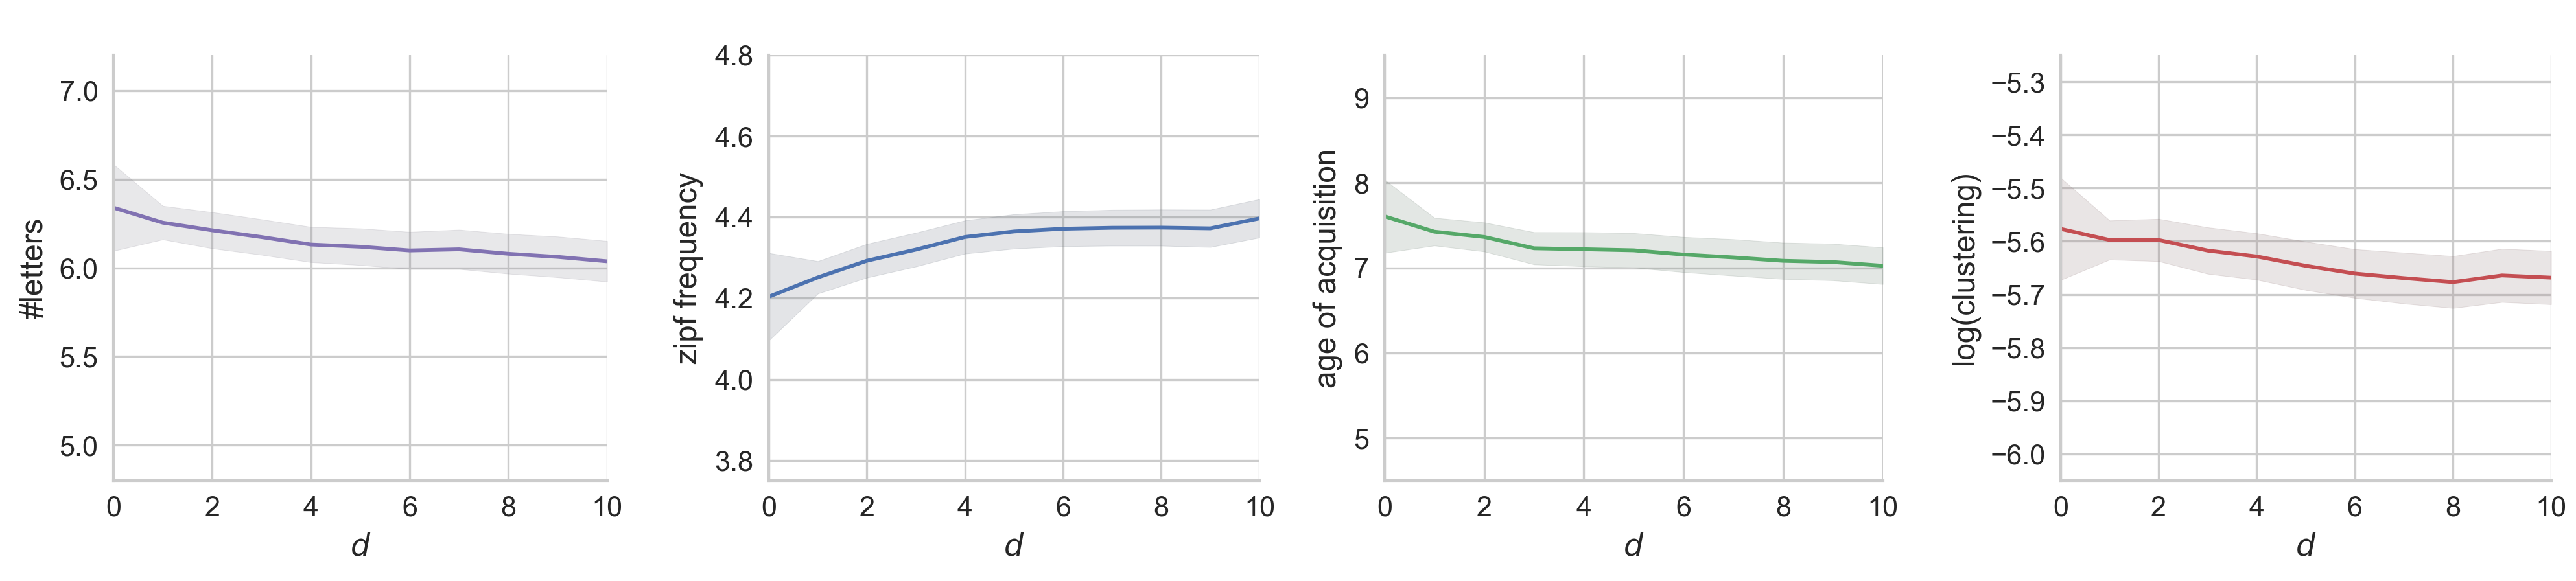
\includegraphics[width=.8\linewidth]{feature-branchevo.png}
	\caption{\emph{Evolution of the average feature values of utterances along transmission chains.}
	Features are \emph{number of letters}, \emph{log-frequency}, \emph{age of acquisition}, and \emph{log-clustering} (a lower clustering value indicates a word that is semantically more differentiated).
	The evolution of each feature corresponds to a drift towards words known for easy recall in laboratory tasks.}
	\label{fig:branchevo}
\end{figure}

More broadly, we argue that this modelling approach provides crucial detail about the transformations, achieving a middle-ground between the focus on lexical features in individual word replacements and the wide-angle view of contrasts in the aggregated evolution of content along chains (the approach commonly taken in transmission chains).
Indeed, it allows us to create a first descriptive model of the transformation of utterances, by bringing together the different base components of a transformation, and quantifying their behaviour and their dependencies.
%Nous proposons alors un premier modèle descriptif de la transformation de ces énoncés en articulant ces différentes composantes entre elles, et en quantifiant le comportement détaillé de chacune d'entre elles.
Such a model, we argue, is an important step forward in creating a bridge between psycholinguistics and the study of cultural evolution.

%\begin{figure}[!ht]
%	\centering
%	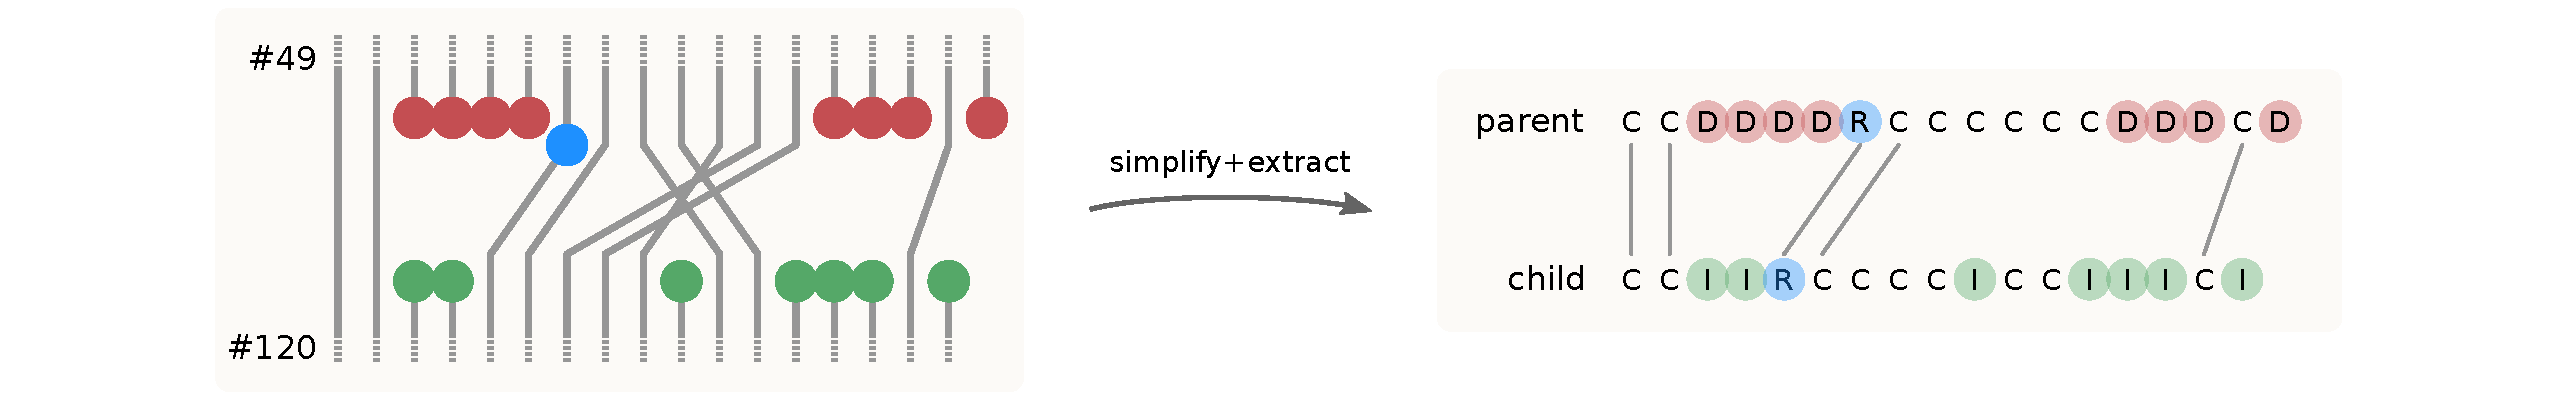
\includegraphics[width=\linewidth]{gistr-utterance-arrays.pdf}
%	\caption{XXX}
%\end{figure}

%Cependant, les effets observés restent au niveau des variables lexicales et des opérations sur des mots, et ne fournissant que peu d'information sur les changements sémantiques opérés par les sujets.
%L'inspection manuelle des données indique que cette question ne sera pas résolue par une simple extension de notre protocole, car elle est bien plus complexe.
%Bien que les motifs identifiés par d'autres études \autocite[par exemple]{lauf_analyzing_2013} sont bien vérifiés ici, on observe également un comportement de type chaotique:
%un changement qui paraît mineur au milieu d'une transformation de plus grande ampleur peut créer des effets comparativement plus grands en aval dans une chaîne, par exemple lorsqu'une ambigüité apparaît et est résolue différemment par l'un des sujets en aval.
%Une accumulation de petits changements peut également mener à un basculement sémantique lorsque les relations entre les mots de différentes sous-parties d'un énoncé sont peu à peu changées.
%Plus généralement, la question des transformations sémantiques nécessite, d'un côté, de définir les niveaux de sens auxquels on s'intéresse, et de l'autre, de questionner le contexte et la tâche dans laquelle une phrase est transformée:
%comme les cas d'évolution chaotique l'illustrent, un changement sémantique peut venir de n'importe quelle ambigüité remarquée par les sujets (une erreur typographique, un changement de ponctuation, ou un changement de vocabulaire en apparence mineur).
%La question ne concerne donc plus seulement la structure syntaxique et lexicale des énoncés, mais aussi la façon dont les sujets portent leur attention sur un énoncé, dans un contexte et une situation d'interaction donnés.
%En d'autres termes, comprendre la façon dont les changements sémantiques opèrent nécessite une analyse de ce qui est pertinent pour un sujet dans une situation donnée, c'est-à-dire une analyse de la pragmatique des énoncés.


\section{Meaning in utterance transformations}
\label{sec:meaning}

So far we have considered the paradigm put forward by Cultural Attraction Theory, and sought to elucidate situations where linguistic representations are transformed as they are transmitted.
We aimed to assess, on one side, the extent to which the empirical evolution of content agrees with what is expected under CAT, and on the other side, the extent to which CAT provides productive guiding questions in understanding what is at work in the situations studied.
%This has led us to identify a number of behaviours which are consistent with Cultural Attraction Theory:
%studying word substitutions in online quotations first, and more general transformations in controlled transmission chains of short utterances second, we showed that the lexical features of words evolve in a systematic manner to make utterances easier to produce, and that the direction of the evolution is consistent with the attraction pattern that can be observed in the individual step of word replacements.
%Le dernier chapitre de cette thèse propose de prendre du recul pour discuter des prérequis à une meilleure compréhension des processus d'évolution culturelle au niveau linguistique.
%Jusqu'ici nous avons considéré le paradigme proposé par la CAT pour identifier et clarifier des situations dans lesquelles des représentations linguistiques sont transformées au fur et à mesure de leur propagation.
%L'objectif a été d'évaluer, d'un côté, à quel point l'évolution observée est en accord avec ce que la CAT prédit, et de l'autre, dans quelle mesure la CAT conduit à des lignes d'exploration productives pour la compréhension des situations que nous avons étudiées.
%Ce faisant nous avons identifié plusieurs motifs compatibles avec les hypothèses de cette théorie.
However, the case studies we presented did not bring us significantly closer to understanding the \emph{semantic} changes that utterances undergo when they are transformed.
In this last chapter we take a broader view on what would be necessary to achieve such a fuller understanding.

%We now wish to discuss the reasons for this limitation.
%Our purpose is first to convince the reader that meaning is a crucial aspect in the evolution of content which must eventually be analysed in order to fully understand the way representations circulate and change.
We begin with a manual exploration of the transformations observed in the previous chapter, showing that the surface measures that we used in quantitative analyses provide only limited insight into the evolution of the meaning of utterances.
Indeed, meaning appears here as a deeply context- and interaction-dependent property which cannot be understood by simply focusing on the utterances themselves;
the lack of a definitive account of utterance meaning in CAT therefore renders the empirical question of attractors in this case under-specified.
%Cependant ces approches n'ont pas apporté d'éclairage sur les transformations sémantiques subies par des énoncés spontanément transformés, que ce soit en ligne ou en expérience contrôlée.
%Cette partie discute donc les raisons de ces limites.
%L'objectif est tout d'abord de persuader le lecteur que le sens, à la fois linguistique et pragmatique, est un aspect central de l'évolution des contenus qui devra à terme être abordé à l'aide d'une théorie complète si l'on veut comprendre la façon dont des représentations circulent et sont transformées.
%Nous commençons donc par détailler plusieurs exemples tirés du deuxième cas d'étude où le sens des énoncés joue un rôle important dans les transformations.
%Ces exemples illustrent en effet comment le sens est une propriété fondamentalement dépendante du contexte et de la situation d'interaction, qui ne peut être comprise en se focalisant uniquement sur les énoncés. 
%% L'étape suivante dans l'explication de l'évolution de tels énoncés à court terme est donc l'analyse des mécanismes d'interprétation des énoncés dans des situations concrètes.
To make progress, we must broaden the scope of empirical studies of CAT beyond interactionless transmission chains and consider all interactions, either face-to-face or digitally mediated, and not necessarily linguistic.
%We are then faced with the concrete question of how to understand the way an agent (human or non-human organism) extracts or constructs meaning in such an interaction.
%That is, which of the infinite possible meanings the agent selects (or constructs), and how that selection (or construction) operates.
%As we just saw, such meaning is highly dependent on the context and interaction the agent finds itself in, such that viable approaches to meaning will necessarily be coping with the complexity of possible interactive situations. This makes the picture considerably more complicated than when dealing with simple context-free utterances.
%Nous avons donc besoin pour avancer d'élargir le champ des études empiriques de la CAT au-delà de chaînes de transmission sans interaction;
%il faut en effet considérer une large palette d'interactions possibles, non nécessairement linguistiques, allant du face à face jusqu'aux interactions au travers d'interfaces numériques.
%Le problème du sens en contexte se pose alors concrètement:
%comment un agent extrait-il ou construit-il du sens à partir d'une interaction donnée?
%En particulier, quel sens, parmi les infinies possibilités disponibles, un agent sélectionne-t-il (ou construit-il), et comment cette sélection (ou construction) opère-t-elle?
%Comme nous l'aurons illustré, le sens dépend fortement du contexte d'interaction dans lequel un agent se trouve, de telle sorte qu'une approche viable risque de se heurter à la complexité des situations d'interaction possibles.
%Le problème devient considérablement plus difficile que dans le cas d'énoncés dénués de contexte.

We therefore discuss two important approaches to studying the meaning of utterances in relation to the context and interaction in which they appear:
Relevance Theory and the Enactive approach.
The first is more mature and better integrated with other areas of linguistics, and has a common philosophical basis with CAT.
It bases its account of meaning on the symbolic processing of mental representations, and fleshes out the idea \autocite[first introduced by][]{grice_studies_1989} that human communication is ostensive communication, based on the recognition of relevant communicative intentions which then enter inference processes in the mind.
The second approach has grown more recently \autocite{cuffari_participatory_2015}, and is philosophically based on authors who have strongly criticised representational approaches to cognition:
it starts from a more bare-bones level of description, and proposes an understanding of meaning as endogenously generated through the interactions of organisms with their environment and other organisms.
It avoids some of the issues with mental representations but has yet to tell a complete story for the study of language.
Both these theories provide (part of) an answer to how agents select, infer or construct subtly varied meanings in the course of an interaction, but they do so by starting from opposite ends and building what is missing for their own account of meaning.
%Relevance Theory starts with representations and symbolic processing, which are implementable in bodies (by following the model of computers) and come already structured in similar ways to language, and constructs on top of those a notion of meaning, with a corresponding interpretation procedure (inference), that is subtle and flexible enough to apply to fuzzy cases like poetry or loose language.
%The Enactive approach starts from an embodied and dynamic notion of meaning, which by definition exists for all organisms and need not be inferred, but comes without any particular structure;
%it then builds its account of language by detailing how interactions (and thus meaning) can become increasingly structured through a series of interactive conventions built on one another.

After a detailed presentation of both approaches and of their relationship to the questions of cultural evolution, we argue that the way forward lies in a healthy pluralism which uses both to explore complementary dimensions of the role of meaning in cultural evolution \autocite[in accordance with][]{chemero_after_2008}, and avoids unnecessary scholasticism.
Indeed, we believe that empirical investigation has an important part to play in such questions, leading us to close the chapter with some informed speculation on concrete experiments that could contribute to the study of meaning in cultural evolution.



%Through a detailed presentation of these approaches, we show that they can be seen as starting from different descriptive levels and building what is missing for an account of meaning:

%Relevance Theory starts with representations and symbolic processing, which are implementable in bodies (by following the model of computers) and come already structured in similar ways to language, and constructs on top of those a notion of meaning, with a corresponding interpretation procedure (inference), that is subtle and flexible enough to apply to fuzzy cases like poetry or loose language.
%The Enactive approach starts from an embodied and dynamic notion of meaning, which by definition exists for all organisms and need not be inferred, but comes without any particular structure;
%it then builds its account of language by detailing how interactions (and thus meaning) can become increasingly structured through a series of interactive conventions built on one another.


%These two approaches illustrate opposite ends of the spectrum of approaches to meaning.

%In this section, we present two prominent approaches to meaning and pragmatics, both of which can prove useful for further exploration of cultural evolution.



%Nous présentons alors deux approches importantes pour l'étude du sens d'un énoncé en lien avec le contexte et l'interaction dans lequel il apparaît:
%la Théorie de la Pertinence et l'Approche Énactive du langage.
%La première théorie, plus mûre et mieux intégrée avec l'ensemble des sujets d'étude de la linguistique, coïncide avec la base philosophique de la CAT:
%elle adopte la métaphore computationnelle de l'esprit, et fonde son explication du sens sur le traitement symbolique de représentations mentales.
%Plus précisément, la Théorie de la Pertinence développe l'idée gricéenne selon laquelle la communication humaine est une communication \emph{ostensible}, basée sur la reconnaissance d'intentions communicatives pertinentes.
%La deuxième approche est plus récente, et sa base philosophique fait appel à des auteurs ayant fortement critiqué les approches représentationnelles de la cognition.
%Elle part d'un niveau de description moins complexe, et développe une explication de la façon dont le sens émerge lors d'une interaction entre deux agents vus comme des organismes dynamiquement couplés.
%Cette notion de sens émergent permet d'éviter certains écueils venant de la notion de représentations mentale, mais ne fournit pas encore une théorie complète pour l'étude du langage.


%The notions of meaning
%to which they arrive are quite different: the first is mechanistic-representational, and the second
%is dynamical, two explanatory approaches that have historically been considered in contradiction.
%However, more recent work suggests that mechanistic and dynamical explanations can be usefully
%combined to describe one same system (Chemero and Silberstein 2008).


%Au travers d'une présentation détaillée, nous montrons que ces deux approches fournissent une réponse (partielle) à la question de comment un agent sélectionne, infère ou construit des significations subtiles et variées au cours d'une interaction, en se basant sur une notion spécifique de pertinence, ou de valeur pour l'agent.
%La Théorie de la Pertinence se base sur une notion propositionnelle des représentations, qu'un agent combine dans un processus de traitement symbolique et d'inférence du sens que l'interlocuteur cherche à communiquer.
%L'ensemble du mécanisme d'inférence peut être implémenté biologiquement (en suivant le modèle d'un ordinateur), et fournit une notion de sens structurée de façon similaire au langage qu'on connaît tout en étant suffisamment subtile et flexible pour s'appliquer à des cas plus difficiles tels que la poésie ou les usages plus libres du langage.
%L'approche énactive ne fait pas appel à des représentations, mais part d'une description d'organismes dont l'interaction et le couplage avec leur environnement est source d'un sens endogène non-représentationnel.
%Par définition, cette notion existe pour tout type d'organisme, est corporisée, ne nécessite pas d'inférence, et s'applique même pour les formes les plus simples d'interaction avec l'environnement.
%En revanche, elle n'a pas de structure propre (à l'inverse d'une représentation propositionnelle);
%l'essentiel de la théorie énactive du langage consiste donc à expliquer comment des interactions, et le sens qui en émane, se structurent progressivement au travers d'une série de conventions émergentes et imbriquées les unes dans les autres.
%Les notions de sens que ces deux approches développent sont donc bien différentes:
%la première est mécanique-représentationnelle, et la deuxième est dynamique.

%Bien que ces deux types d'explications et de notions soient traditionnellement considérées comme diamétralement opposées, nous choisissons de laisser de côté le débat visant à trancher en faveur de l'une ou de l'autre.
%En accord avec certains travaux récents \autocite{chemero_after_2008}, nous défendons un certain œcuménisme consistant à identifier les compatibilités entre ces deux approches:
%toutes deux peuvent servir de guide utile et productif pour l'exploration empirique du sens en contexte, et il nous semble donc plus judicieux d'encourager une démarche permettant de faire avancer l'ensemble du champ en tirant parti de toutes les options qui s'offrent à elle.
%Une telle démarche peut en effet jouer un rôle crucial pour la question du changement culturel sémantique.

%Enfin, nous terminons le chapitre en esquissant trois grandes possibilités de travaux empiriques futurs, permettant de progresser par l'application de certains principes des approches détaillées précédemment.
%La première possibilité est une méthode d'analyse du sens directement applicable au cas d'étude présenté dans le chapitre précédent, basée sur une évaluation de triplets d'énoncés sous-traitée à des codeurs externes.
%La deuxième piste consiste à introduire une mesure de l'interaction et du contexte par doses progressives dans des paradigmes expérimentaux existants:
%c'est possible à faible dose pour un paradigme similaire à celui d'une chaîne de transmission, ou à forte dose dans des situations où le contexte est intégralement mesuré (par exemple un lieu de vie entièrement filmé et enregistré), puis analysé au moyen d'un codage quali-quantitatif.
%La dernière piste consiste à étendre le travail empirique déjà effectué dans le cadre de l'approche énactive du langage, afin d'avancer dans la structuration des interactions étudiées et ainsi accroître la complexité du sens que cette approche est capable d'expliquer.

%Favouring one or the other, or possibly combining parts of the two, will undoubtedly be related to one's overall construal of cultural evolution and to the importance of representations in a theory of cultural change;
%we will not venture into that territory however, and will limit ourselves to exposing alternatives available to empirical approaches.
%Indeed, we believe that informed empirical investigation has an important part to play in the question of meaning in cultural change and the debates it relates to.
%After having laid out these two alternatives, then, we propose some speculation on practical approaches that could contribute to the empirical side of this question.
%Finally, we present possibilities for advancing the debate through empirical investigation.


\section*{Conclusion}
\label{sec:conclusion}

Taken together, we believe these works provide a significant step forward in empirical approaches to the study of short-term cultural evolution:
they fill gaps in the current empirical exploration of CAT, detail two novel techniques that could be fruitfully reused and extended to improve empirical prospects, and extend further proposals for the semantic understanding of transformations.
More proximally, they also create an accurate picture of the way written utterances are transformed in chains, providing a partial answer to how linguistic content might evolve as it spreads through a social network.
%Considérés dans leur ensemble, nous pensons que les travaux présentés ici constituent une avancée substantielle dans l'étude empirique de l'évolution culturelle à court terme:
%ils répondent à plusieurs lacunes dans l'exploration empirique de la CAT, et fournissent deux nouvelles méthodes qu'il serait utile d'appliquer et d'étendre à d'autres situations.
%Ils fournissent également une vue détaillée de la façon dont des énoncés sont transformés lors de leur transmission en chaîne, apportant des éléments importants dans la compréhension de l'évolution de contenus linguistiques au cours de leur diffusion dans un réseau social.

%Le développement de modèles comme celui présenté au chapitre \ref{sec:gistr} permet également de progresser non seulement sur la question de l'évolution culturelle et linguistique, mais également vers le débat autour des liens entre évolution culturelle et théories du sens.
%En somme, nous pensons qu'une exploration empirique telle que celle présentée ici peut être extrêmement utile pour améliorer notre compréhension de l'évolution culturelle et sémantique, qu'elle soit à court ou à long terme.


\printbibliography[title=Bibliography]

\end{document}
